%-------------------------------------------------------------------------------
% Preamble
%-------------------------------------------------------------------------------

\documentclass[a4paper, 12pt]{article}
\usepackage{ms}            % load the template
\usepackage[osf]{mathpazo} % palatino
%\usepackage[round]{natbib} % author-year citations
\usepackage[superscript,biblabel]{cite} % for superscript citations
\usepackage{graphicx}
\usepackage{subcaption}
\usepackage{parskip} 
\usepackage{amsmath}
\usepackage{longtable}
\usepackage{pdflscape}

\pagenumbering{arabic}  
\linespread{1.66}

%-------------------------------------------------------------------------------
% Title page information
%-------------------------------------------------------------------------------

\title{Sex biases in bird and mammal natural history collections}

\author{
  Natalie Cooper$^{1*}$, 
  Alexander L. Bond$^{1,2}$,
  Joshua L. Davis$^{1}$,\\
  Roberto Portela Miguez$^{1,3}$,
  Louise Tomsett$^{1,3}$,\\ and 
  Kristofer M. Helgen$^{1,3,4}$, 
}
\date{}
\affiliation{\noindent{\footnotesize
  $^1$Department of Life Sciences, Natural History Museum, Cromwell Road, London, SW7 5BD, UK.\\
  $^2$Bird Group, Department of Life Sciences, Natural History Museum, Akeman Street, Tring, Hertfordshire, HP23 6AP, UK.\\ 
  $^3$Mammal Group, Department of Life Sciences, Natural History Museum, Cromwell Road, London, SW7 5BD, UK.\\
  $^4$Department of Ecology and Evolutionary Biology, School of Biological Sciences, University of Adelaide, North Terrace,  Adelaide, SA 5005, Australia.\\
  $*$Email address: natalie.cooper@nhm.ac.uk
}}

\vfill

\runninghead{Sex biases in collections}
%\keywords{}
%}

%-------------------------------------------------------------------------------
% Begin document
%-------------------------------------------------------------------------------
\begin{document}
\modulolinenumbers[1]   % Line numbering on every line

\mstitlepage

\parindent = 1.5em
\addtolength{\parskip}{.9em}

\raggedright
%-------------------------------------------------------------------------------
% Abstract
%-------------------------------------------------------------------------------

\section{Abstract}

Natural history specimens are widely used across ecology, evolutionary biology, and conservation.
Although biological sex may influence all of these areas, it is often overlooked in large-scale studies using museum specimens. 
If collections are biased towards one sex, studies may not be representative of the species. 
Here, we investigate sex ratios in over two million bird and mammal specimen records from five large international museums. 
We found a slight bias towards males in birds (40\% females) and mammals (48\% females), but this varied among orders. 
The proportion of female specimens has not significantly changed in 130 years, but has decreased in species with “showy” male traits like colourful plumage and horns. 
Body size had little effect. 
Male bias was strongest in name-bearing types; only 27\% of bird and 39\% of mammal types were female. 
These results imply that previous studies may be impacted by undetected male bias, and vigilance is required when using specimen data, collecting new specimens, and designating types.

\textbf{Keywords: sex bias, museum specimens, natural history collections, birds, mammals}

%-------------------------------------------------------------------------------
% Main text
%-------------------------------------------------------------------------------

\section{Introduction}\label{main}
Museum specimens are used extensively in studies of taxonomy, systematics, biogeography, genomics, comparative anatomy, morphological variability, development, parasitology, stable isotope ecology, toxicology, morphological evolution and more\cite{lister2011natural,pyke2010biological,mclean2015natural}. 
They are also of vital importance for understanding how biodiversity responds to anthropogenic impacts\cite{meineke2018biological}. 
Large studies of species phenotypes using museum specimens, especially in vertebrates, are becoming increasingly common (e.g. evolutionary dynamics in birds\cite{cooney2017mega}, ecomorphological diversification in squamates\cite{watanabe2019}) and are revealing new insights into the evolution of diversity. 
These studies require large amounts of data, which can mean the focus is on collecting data from as many species as possible, to the detriment of other sources of variation. 
Sex is an important factor that influences many aspects of an individual's ecology and life-history (Table \ref{table_consequences}), but it is often treated as a nuisance variable, overlooked entirely, or data collection focuses on just one sex (e.g. only measuring female rates of phenotypic evolution\cite{cooper2009factors}) to avoid the issue. 
If natural history collections have unbiased sex ratios (i.e. close to 50\% males and females, or reflective of the sex ratio for the species in the wild\cite{karlin1986theoretical}) then this may not be a problem; if there is a bias in the sex composition of collections, this has implications for studies that assume their samples are representative of the whole population or species (Table \ref{table_consequences}). 
No large-scale study of sex ratios in bird and mammal museum collections exists, therefore investigating this is of vital importance as the number of studies using museum specimens continues to rise (e.g. this recent special issue on using museum specimens to study biodiversity in the Anthropocene\cite{meineke2018biological}).

\newpage
\begin{landscape}
  % Table 1

\begin{longtable}{p{3cm} p{16cm}}

\caption{Prominent uses of natural history specimens and how research outcomes may be influenced by sex biases.}\\ 
  
  % Header
  \hline
  \textbf{Use} & \textbf{Might sex biases in birds and mammals affect research outcomes?}\\ 

  % Body of table
  \hline
  Taxonomy & \textbf{Yes}. Sexes often have external differences; if these are used in the taxonomy of the group (e.g. male plumage colouration in birds\cite{paxton2009utility}) then it may be more difficult to identify individuals to species-level in one sex than another. Consistent over-representation of one sex in samples used in taxonomic studies, and in selection of name-bearing types in particular, may mean that interspecific distinctions between taxa are framed most often for that sex, making the less-represented sex harder to identify and distinguish across species, even if important differences exist, a considerable practical problem. \\ 

  Systematics & \textbf{Maybe}. For standard molecular phylogenies, commonly used genes do not differ substantially among sexes (i.e. not to the extent that they would form different branches). In phylogenomic studies, however, gene trees may vary across a genome if sex chromosomes are included in the sample\cite{reddy2017}. Morphological phylogenies are likely to be most affected, as morphological characters can vary extensively between males and females. This also has implications for Total Evidence phylogenies that use both morphological and molecular data. mtDNA is often used to investigate species limits (e.g. gentes limits in cuckoos\cite{soler2009geographic}) and this may differ across sexes.\\ 

  Biogeography & \textbf{Maybe}. This depends on the scale at which you consider biogeography. In species where all reproduction is sexual, sexes (necessarily) do not differ in terms of large-scale historical biogeography, i.e. colonisation of new regions will not succeed if only one sex colonises. However, locally sexes may be spatially segregated (e.g. bat roosting sites\cite{altringham}), and have different dispersal rates\cite{pusey1987sex} or patterns of habitat use, and differential migration of sexes is common in birds\cite{Woodworth2016}.\\ 

  Genomics & \textbf{Yes}. Mammals and birds have chromosomal sex determination; in mammals XY male and XX female, in birds ZZ male and ZW female\cite{stevens1997sex}. The X and Z chromosomes are larger and have more genes than W and Y, thus genome size differs among sexes. Many genes are also sex-linked, so genomes will differ between sexes.\\ 

  Comparative anatomy & \textbf{Yes}. Males and females have internal and external anatomical differences, thus sex biases will influence comparative anatomy studies.\\ 

  Development & \textbf{Maybe}. In most vertebrates, early developmental stages are almost identical in males and females, however later development and sexual maturation involve highly divergent growth to result in adult sex differences\cite{badyaev2002growing}. If research is focused on early development or juvenile life-history stages then sex biases are unlikely to pose a problem.\\

  Morphological variability & \textbf{Maybe}. Perceived wisdom is that males are more variable than females. However, many detailed morphometric studies do not find this (e.g. in mammalian dentition and skull variation\cite{polly1998variability,biswas2019} and references within) in birds or mammals when a large sample is included. In some groups females are more variable than males (e.g. in \textit{Pyriglena} antbirds\cite{isler2017calls}).\\ 

  Parasitology & \textbf{Yes}. Males are commonly more susceptible to infection, have lower immune function, and higher parasite loads than females\cite{zuk2009sicker}. This is likely due to testosterone inhibiting the immune system\cite{Klein:2016aa}. However, this is not true for all species and all kinds of parasites, e.g. breeding female birds have more blood parasites than males\cite{mccurdy1998sex}. Differences in either direction may cause parasite load and diversity to be misrepresented where collections are sex biased.\\ 

  Stable isotope ecology & \textbf{Yes}. The demands of producing eggs, brooding, pregnancy, and lactation can alter stable isotope ratios\cite{fuller2004nitrogen}. Many species also have sex segregated diets, e.g. leopards\cite{voigt2018sex}, and foraging ranges, so stable isotope ratios may vary among sexes even in non-breeding individuals.\\ 

  Toxicology & \textbf{Yes}. As above, sexes may differ in foraging ecology, which has consequences for contaminant burden. Furthermore, females may be able to eliminate some contaminants via eggs (e.g. mercury\cite{robinson2012sex}), an option not available to males.\\ 
  Morphological evolution & \textbf{Yes}. There is extensive sexual dimorphism in many of the traits used in studies of morphological evolution, for example body size\cite{Uyeda15908}, thus tempo and mode of evolution may vary with sex.\\ 

  \hline
\label{table_consequences}
\end{longtable}


\end{landscape}

Here we investigate sex biases in natural history collections of birds and mammals using over two million specimen records from five major international museums.
We find a slight bias towards males in both groups.
Curators and collections managers do not as a rule discard specimens based on sex, thus any bias is likely related to what is collected in the field. 
Male bias may be related to active selection for males by collectors in the field, or active avoidance of females with young due to legislation, ethical or conservation considerations. 
In particular a major suspected source of male bias in collections for some species is deliberate selection for large, ``impressive'' male specimens, especially where males are larger or more colourful than females, or possess ornaments or weaponry such as horns or antlers.
Given the age of most major natural history collections, some male bias may be related to the changes in attitudes towards sex through time, therefore, we expect male bias to decrease towards the present due to changes in collection methods and motivations over the last century. 
Alternatively, male bias may be accidental, for example due to trapping biases (i.e. trapping method, season of collecting, conspicuous male behaviors or traits), difficulties identifying females to species-level, or in some cases simply because there were more males in a population. 
In some mammals, higher dispersal, and broader habitat use, in males may result in them being more likely to come into contact with hunters or traps; males may also exhibit lower levels of neophobia increasing their likelihood of being captured, though evidence for this is limited\cite{crane2017patterns,laviola1992sexual}. 
In some birds, male territorial calls are often used to bring individuals towards a trap, which may also bias collections towards males.

To investigate these biases further, we tested whether male bias differed among orders, with sexual size dimorphism, with the possession of colourful plumage (birds) or ornamentation or weaponry (mammals) in males, and through time. 
Note that these variables mostly test for deliberate selection for males, because these data are easier to collate, but our results are likely a combination of deliberate and accidental male biased collecting.

\section{Materials and Methods}
\subsection{Data collection and cleaning}
\subsubsection{Specimen data} 
We obtained museum bird and mammal collection records from the Global Biodiversity Information Facility (GBIF\cite{gbif}). 
Specifically we collated data from the American Museum of Natural History (AMNH; $n = 271,407$ records\cite{amnh-birds,amnh-mammals}), Field Museum of Natural History (FMNH; $n = 182,984$ records\cite{fmnh-birds,fmnh-mammals}), Mus\'{e}um National d'Histoire Naturelle (MNHN; $n = 86,126$ records\cite{mnhn-birds,mnhn-mammals}), National Museum of Natural History, Smithsonian Institution (NMNH; $n = 496,735$ records\cite{smithsonian-both}), and Natural History Museum, London (NHMUK; $n = 251,409$\cite{nhm-all}).
These specimens were obtained between 1751 and 2018, mostly through hunting or trapping, and sexed based on internal or external genitalia or secondary sexual characters, for example plumage colouration or antlers.
All raw data can be downloaded from GBIF\cite{gbif}.
 
Prior to analyses we cleaned the data as follows. 
(i) Record type. To avoid confusing specimens with archives describing specimens we selected only preserved specimen records; 
(ii) Age. Juveniles can be harder to sex so we excluded all juveniles, young and foetuses from the dataset; 
(iii) Year. We removed collection years later than 2018 as these were clearly errors; 
(iv) Taxonomy. We removed subspecies names and used species binomials because we were interested in species-level sex ratios. 
To ensure our results were not due to female specimens more frequently being identified to the genus-level only, we also also created a dataset with all specimens with valid generic names.
We corrected bird taxonomy using the GBIF backbone taxonomy\cite{gbif}, and mammal taxonomy using Mammal Species of the World\cite{wilson2005mammal}; 
(v) Type status. We split types into name bearing (Holotype, Syntype, Lectotype, Neotype) and non-name bearing (all others) types. Where the records did not specify the kind of type we define these as ambiguous types; 
(vi) Sex. We standardized sex to either Female, Male or non-sexed, and removed intersex or hermaphrodite individuals. 
Note that we recognise that biological sex is a spectrum\cite{sciam2017}. 
We focus here on specimens identified as females and males for simplicity because there were very few recorded intersex specimens in collections databases (only five remained after other data cleaning), but we recognize the importance of these individuals.
We also excluded non-sexed individuals from the analyses.
The final dataset contained 2,496,611 specimens (1,395,748 birds and 1,100,863 mammals), 1,647,409 (708,355 birds and 939,054 mammals) of which were sexed (Table A1).

\subsubsection{Sexual dimorphism, plumage colouration and ornamentation data.}
We extracted median body masses (g) for males and females from Lislevand et al.\cite{lislevand2007avian} for birds and Jones et al.\cite{pantheria} for mammals, then calculated sexual size dimorphism by dividing mean male body mass by female body mass. 
Note that the sample size for these variables is lower because sex disaggregated body size data are rare (see Table A2).

To explore how ``showiness'' might influence sex bias, we included a measure of plumage colouration for passerine birds taken from Dale et al.\cite{dale2015data,dale2015effects}. 
This measure is based on the mean RGB (red green blue) values for 400 randomly chosen pixels in six patches (nape, crown, forehead, throat, upper breast, and lower breast) for each sex. 
We then calculated a plumage dimorphism score by dividing male plumage score by female score for each species. 
For mammals, we used the Handbook of Mammals of the World to identify mammals where males have ``ornamentation''. 
We defined ornamentation as a feature that might increase the likelihood of a collector targeting an individual, specifically horns, antlers, tusks, well-defined manes (i.e. in lions and some baboons), enlarged nasal appendages (e.g. in elephant seals, proboscis monkeys and hammerhead bats), facial colouration (e.g. in mandrills) or large cheek extensions (e.g. orangutans). 
Where species had ornaments, we recorded whether both sexes or only males routinely possess them. 
Note that the majority of species with ornaments in our models were Artiodactyla (59 of 67 species). 

Bird species in several groups show reverse sexual dimorphism, where females are larger or showier than the males. 
To see if we detect a different pattern in these species we also divided the bird data into species where the female is generally the larger or showier sex (the families  Accipitridae, Falconidae, Scolopacidae, Charadriidae, Jacanidae, Stercorariidae, Sulidae, Fregatidae, Cuculidae, Trochilidae, Pipridae, and the orders Strigiformes and Struthioniformes - list taken from\cite{swaddle2000novel}), and species where the male is generally the larger or showier sex (all other species). 

The final cleaned data are available on the NHM Data Portal \cite{sex-bias-data}. 

\subsection{Analyses}
We analysed bird and mammal data separately and performed all analyses in R version 3.5.0\cite{R}. 
Reproducible scripts are available on GitHub at https://github.com/nhcooper123/sex-bias-museums\cite{coopercode2019}.

We first summarised the overall proportion of female, male and unsexed specimens, and calculated the median proportion of females across species (using the main species-level dataset) and genera (using the generic-level dataset). 
We then summarised differences in the proportion of female specimens across orders and types. 

Unsexed specimens may bias our results toward males if the majority of unsexed specimens are female. 
We tested for this by fitting linear models to compare the percentage of unsexed specimens and the percentage of female specimens within species; if these unsexed specimens are generally female we expect to see a negative relationship between unsexed specimens and the proportion of females in a species. 
In addition, we investigated variation in the numbers of unsexed specimens by order, collection continent and collection decade (see Supplementary Materials).

Most species were represented by only a few specimens (Figure A1), with large skews towards either males or females at low numbers (Figure A2). 
To reduce problems this is likely to cause when fitting models, we used only species with 100 or more specimens in our models (see Supplementary Materials for more details), except in our change through time models. 
In these models our response variable was the proportion of males and females in each species for each year from 1880-2010 (before 1880 and after 2010 we did not have any species with sufficient specimens to include). 
As there were only 55 bird species and 1,216 mammal species with over 100 specimens in a year, change through time models instead used all species with more than 50 specimens in a single year to increase the sample size (see Table A2).

We fitted all models using generalised linear models (GLM) with quasibinomial errors, with the proportion of female specimens (success) and the proportion of male specimens (failure) for each species as the response variable (i.e. a binomial response where the number of females and the number of males for each species were jointly modeled). 
Quasibinomial rather than binomial errors were used due to overdispersion (all models have deviance/residual degrees of freedom far greater than two; see output on GitHub for exact values), and we assessed the significance of model terms using Type II sums of squares. 
We used standard model checks for GLMs (Q-Q plot, histogram of residuals, residuals vs. linear predictors, response vs. fitted values) to assess model fit. 
We tested whether the proportion of female and male specimens varied with (i) orders; (ii) collection years (1880-2010); (iii) male body mass (log transformed); (iv) sexual size dimorphism (log transformed); (v) whether males were larger/more showy than females or vice versa (reverse sexual dimorphism; birds only); (vi) plumage dimorphism (log transformed; passerine birds only); and (vii) ornamentation (mammals only). 
The number of specimens and species in each model are shown in Table A2.

\section{Results and Discussion}

Of the 2,496,328 specimen records (1,395,748 birds and 1,100,580 mammals) in our dataset, 20\% of bird specimens were female, 31\% were male, and 49\% were not sexed (Table A1). 
For mammals, the number of non-sexed individuals was much lower at 15\%, likely because it is often easier to identify sex in mammals, with 41\% female and 44\% male specimens. 
If we consider only sexed specimens, 40\% of bird and 48\% of mammal specimens were female (Figure A3). 
In real terms this represents 143,905 more male than female specimens in birds and 40,468 more male specimens in mammals. 
This male bias was not due to unsexed specimens mostly being female (see Supplementary Materials; Figures A4-A8).
Results were also qualitatively similar using the generic-level data (Table A1), so we focus only on species-level data below.

In the wild, adult sex ratios in many bird species are male skewed, though on average not as skewed as our results (n = 187 species, median 44.8\% female\cite{szekely2014sex}; see Supplementary Materials; Figure A9), however, 48\% is not a large deviation from the 50\% expected in many natural populations of mammals\cite{karlin1986theoretical}.
Well sampled species (i.e. those with at least 100 specimens) with the most extreme sex ratios in our data, i.e. species with fewer than 25\% female or 25\% male specimens, are shown in Table A3.

\subsection{Variation among orders.} 
The proportion of female specimens varied across orders for both birds ($F_{24, 1721} = 29.81$, $p < 0.001$; Figure \ref{fig-bird_order_six}; Figure A10; Table A4) and mammals ($F_{24, 1488} = 19.80$, $p < 0.001$; Figure \ref{fig-mammal_order_six}; Figure A11; Table A4). 
Most orders had more males than females (Table A4). 
In birds, of the 25 orders with sufficient data, only tinamous (Tinamiformes; 50.4\%) had more females, but these represented just four species in the dataset. 
The most male-biased orders with more than 25 species were pigeons and doves (Columbiformes; 36.8\% female), hummingbirds and swifts (Apodiformes; 37.2\%; but see Supplementary Materials; Figure A12), and passerines (Passeriformes; 38.4\%). 
Adult sex ratios in Columbiformes and Passeriformes are generally male-skewed\cite{szekely2014sex,bosque2019skewed,mayr1939sex}, but hummingbirds are often female-skewed in the wild\cite{szekely2014sex,mayr1939sex}. 
This, along with evidence that, on average, Passeriformes are not as male biased as our results ($n = 54$ species, median 45.1\% female\cite{szekely2014sex}), suggests that greater availability of males alone cannot account for our results.

Seven of the 25 mammalian orders with sufficient data had more females, the most extreme being anteaters and sloths (Pilosa; 71.1\% female). 
Most mammal species have a sex ratio of 1:1 at birth\cite{karlin1986theoretical}, though this can vary in adults. 
Several species of sloth have higher numbers of females (up to 68.8\% females\cite{reyes2015informacion}) which may explain why we also found more females in collections, however, giant anteaters (\textit{Myrmecophaga tridactyla}) show variable sex ratios in the field\cite{anteater2005}, but strong female bias in collections (71.3\% female). 
Among the orders represented by more than 25 species in our data, only bats have more females (Chiroptera; 52.2\% female; Figure \ref{fig-mammal_order_six}), despite reportedly balanced adult sex ratios in the wild\cite{altringham}. 
This is likely related to widespread sex segregation in bat roosting sites, with many roosts containing individuals of only one sex\cite{altringham}. 
In the the past, bats were often trapped by collecting all individuals in a roost site, and female bats may use fewer roost sites than males (e.g. in \textit{Myotis daubentonii}\cite{encarnaccao2012spatiotemporal}), so skew towards females is not surprising. 
The most male-biased order of mammals were the even-toed ungulates (Artiodactyla; 39.7\% females), but although they exhibit a great deal of variation in adult sex ratio, on average, there are more females than males in wild populations\cite{berger1999sex} suggesting strong selection for male specimens in this order derived from the deliberate hunting of large males that was common in the 19th and early 20th centuries.

\subsection{Changes through time.}
We found male bias increased for birds ($F_{1, 389} = 7.167$, $p = 0.008$; Figure A13), but decreased for mammals ($F_{1, 3426} = 6.86$, $p = 0.009$; Figure A13), however the effect sizes were extremely small (birds: $slope \pm SE = -0.002 \pm < 0.001$; mammals: $slope \pm SE = 0.001 \pm < 0.001$), indicating very little change in either class, i.e. there has been no improvement in the sex balance of collecting over the last 130 years.

\subsection{Male body mass and sexual size dimorphism.}
We found significant effects of male body size on the proportion of female specimens in both birds and mammals (Table A5), however, the direction and strength of the relationship varied among classes and orders (Figures A14-A16; Table A5).
Bird species with larger males tended to have more female specimens, whereas the reverse was true for mammals. 
In mammals this was likely driven by a few orders with large males that have long been favored in collections (e.g. Artiodactyla, Carnivora) and have low median percentages of female specimens (Figure \ref{fig-mammal_order_six}; Table A4). 
Interestingly however, selection for males in these groups did not increase with increasing male body size (Figure A16), instead it appears male carnivores and artiodactyls were preferred over females, regardless of their body size.

Rather than selecting large males \textit{per se}, collectors may favour males when the difference in size between females and males, i.e. sexual size dimorphism, is large. 
We found that as sexual size dimorphism increased, i.e. as males became increasingly larger than females, there was more bias towards male specimens (Table A5), however, this result was entirely driven by differences among orders (Figures A17-A18); when order was included in the models, sexual size dimorphism did not significantly influence specimen sex ratios over the effects of order (Table A5). 
As with body mass, this suggested certain orders were more likely to contain more male specimens, regardless of their size with respect to females, suggesting that other characteristics were driving their selection.

In birds that show reverse sexual dimorphism we found that the median percentage of females for species where the male was the larger or showier sex was 40\%, the same as for the whole dataset. 
For species where the female is the larger or showier sex the median percentage of females was 44.6\%, closer to the expected 50:50 ratio.
 There were significantly more females in species where the female is the larger or showier sex ($F_{1, 1744} = 167.9$, $p < 0.001$; Figure A19).

\subsection{Plumage and ornaments.} 
In passerine birds, as males became increasingly more colourful than females, the proportion of female specimens decreased (Figure \ref{fig-plumage}; $F_{1, 828} = 58.95$, $p < 0.001$; $slope \pm SE = -0.416 \pm 0.054$). 
This relationship was not strong, but fits with anecdotal evidence of collectors preferentially selecting colourful male specimens, especially where plumage differences are large, for example in birds of paradise. 
Although the numbers are too small to drive the differences seen here, there is also bias towards displaying male specimens in exhibits\cite{machin2008}.

For mammals, species with ornaments (horns, antlers, tusks, manes etc.) had significantly fewer female specimens than those without ornaments (Figure \ref{fig-orn}; $F_{1, 1510} = 46.98$, $p < 0.001$; $slope \pm SE = -0.328 \pm 0.048$). 
Note, however, that only 67 species across four orders in our analyses had ornamentation (Table A6).
Most of the species with ornaments in our models were artiodactyls, and most artiodactyls have horns, antlers or tusks, suggesting that the strong male bias in Artiodactyla (39.7\% female; Figure \ref{fig-mammal_order_six}) was due to selection for males with these features. 
Within ornamented species there was no significant difference if both sexes or only males possessed the ornament (Figure \ref{fig-orn}; $F_{1, 65} = 0.725$, $p = 0.398$), suggesting that even where females are phenotypically different, preference is still given to collecting males. 
This is particularly concerning since most artiodactyl species are female skewed in the wild\cite{berger1999sex}. 
We note, however, that artiodactyls only make up 4\% of our dataset, and just over 4\% of all mammal species\cite{wilson2005mammal}, so while deliberate hunting of large males may be a driver in this order, it is unlikely to drive all male biases we see.

\subsection{Type specimens.} 
Perhaps our most notable finding focused on name bearing type specimens (holotypes, syntypes, lectotypes, and neotypes). 
Here the bias towards male specimens was extreme; only 25\% of bird and 39\% of mammal types were female (Figure A3). 
Although in some instances, males might be considered the appropriate sex for holotypes because male characters such as plumage or bacula are diagnostic (e.g. in bats\cite{bacula}), we see no reason to not also designate a female paratype to represent the phenotypic range of a species - with the exception that in rare species, or species with few specimens for another reason, this may not be possible.
In mammals paratypes were almost 49\% female, but bird paratypes were 38\% female. 
Additionally, for newly discovered species, genetic identification of species limits may remove the need for male diagnostic characteristics, and thus male holotypes. 
Currently sex does not form any part of the International Code for Zoological Nomenclature (ICZN) recommendations for designating types, although some historical instructions for collectors emphasize the importance of multiple types (e.g. the classical description of the type\cite{schuchert1897type}). 
Adding this to the ICZN is of vital importance moving forwards.

\subsection{Conclusions and recommendations.}
Here we tested for deliberate selection of large, showy males, especially in species with high levels of sexual dimorphism in these traits.
Our analyses suggest that some male bias in collections is the likely result of historical active selection of males.
In mammals, males are favoured in species with larger males, and in species with ornaments. 
These results, however, are driven by carnivores and artiodactyls, and do not account for male biases in species which are not actively targeted by hunters, for example most rodents. 
In birds, showier males appear to be favoured within passerines, and species that exhibit reverse sexual size dimorphism show less bias towards males.
As passerines make up 58\% of our dataset (and around 60\% of all bird species), active selection for males may be a much larger problem in birds than in mammals.
To reduce these imbalances, collectors in the field should strive to avoid trapping biases and biases in selecting individuals to collect.

Much bias towards males is probably non deliberate, and related to the characteristics of individual species and how they are trapped. 
In small mammals, for example, higher dispersal and broader habitat use in males may result in males being more likely to come into contact with hunters or traps\cite{pusey1987sex}. 
In passerines, male calls are often used to draw birds towards a mist net, resulting in higher numbers of males being trapped (a simple solution to this is to also use playback of female calls, an active area of current research in ornithology\cite{femalebirds}).
Some trapping is also opportunistic, so characteristics that mean one sex is exposed to collectors more often may play a key role.
For example, the slight female bias in Tinamiformes (50.4\%) in this study may be because they are often collected on their nests. 
Similar patterns are likely for other conspicuous ground-nesting birds.
Differential migration of sexes may also influence the numbers of males and females caught at certain locations throughout the year\cite{Woodworth2016}.
More ecological studies on species with strong biases towards males or females are needed to help explain these patterns.
On top of these factors, females may be harder to identify than males - they may appear similar to juveniles, or lack diagnostic features such as bacula that make identification simpler.
If this is the case, many of our unsexed specimens may be female. 
Our supplemental analyses (Figures A4-A8) suggest this does not cause the male bias, but until these 687,393 unsexed bird and 161,526 unsexed mammal specimens are sexed, we cannot determine it would have no effect.

Museum professionals, and those using museum collections, should have an awareness of the biases within their collections (not just in terms of sex but also in terms of age, locality, and other factors), and attempt to acquire material to best resolve those biases, whatever their cause. 
Natural history collections play a critical role in informing multiple research disciplines answering vital questions for the future of biodiversity\cite{meineke2018biological} and are also key resources for public engagement and interaction with biodiversity\cite{machin2008}. 
Therefore it is paramount that we continue developing these resources while using a more comprehensive and better informed approach. 
Finally, researchers investigating broad-scale variation in species should account for these biases when designing data collection protocols and/or in downstream analyses and declare how they dealt with those biases in resulting publications. 
Our analyses place particular pressure on taxonomists to think more carefully about sex when defining name-bearing types, and suggest more designation of opposite sex paratypes would be desirable, particularly in birds. 

\section{Acknowledgments}
We thank all collection managers for inputting specimen data to GBIF, and two anonymous reviewers for insightful comments on an earlier version.

\section{Data accessibility}\label{data-code-and-materials}
Data are available from the NHM Data Portal \cite{sex-bias-data} and GBIF\cite{gbif}. 
R code is available from GitHub (https://github.com/nhcooper123/sex-bias-museums; Zenodo DOI: 10.5281/zenodo.3459138).

\section{Funding}
This work was not supported by any grant funding.

% References
\bibliographystyle{bibstyle}
\bibliography{sex-bias}

\section{Author contributions}
NC performed the analyses and wrote the first draft. All authors contributed to study design, interpreted results, revised the manuscript, and approved the submitted version.

\section{Competing interests}
The authors declare no competing interests.

\section{Figures}

% figure 1
\newpage
\begin{figure}[h]
 \centering
  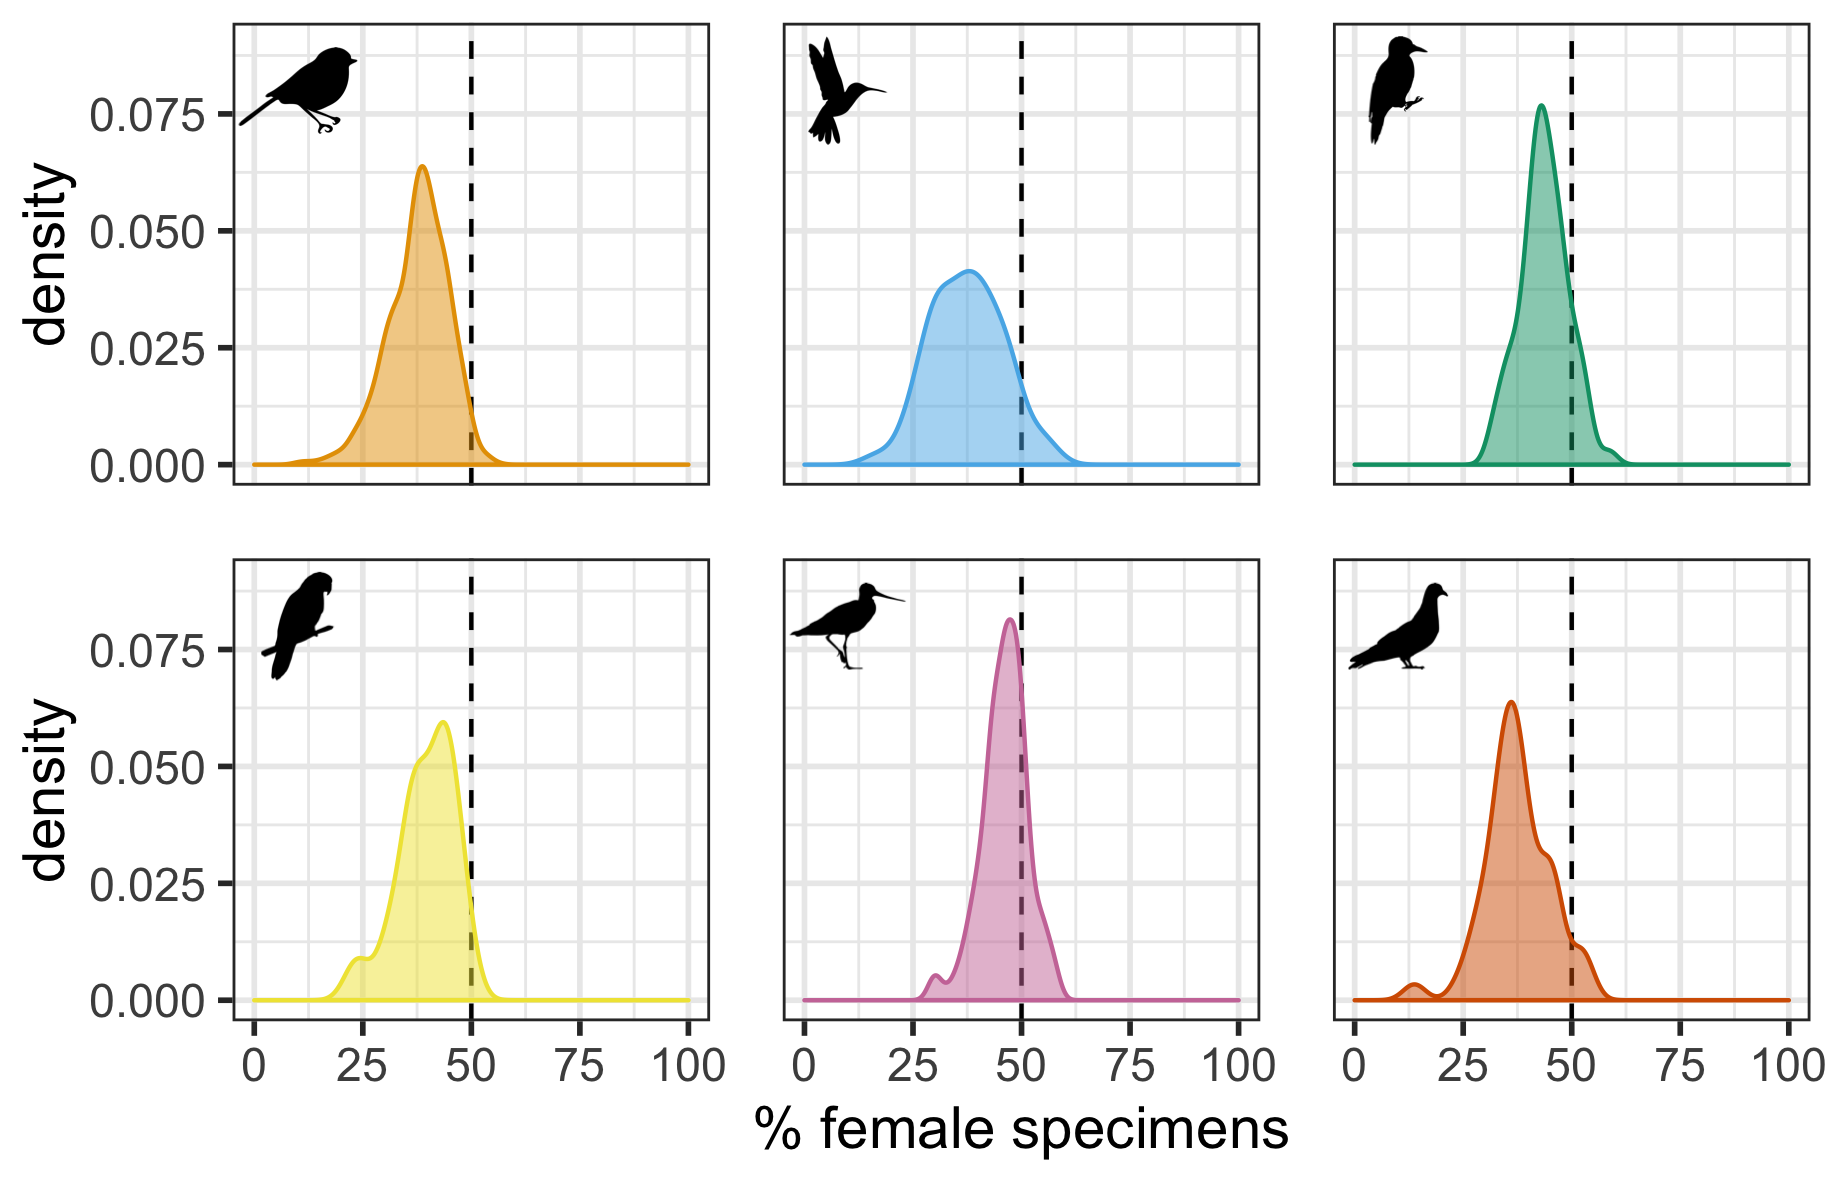
\includegraphics[width = \linewidth]{figures/orders-density-birds-six.png}
  \caption{Kernel density plots showing the \% female specimens in each species across the six largest orders of birds (from left to right, top to bottom: Passeriformes, Apodiformes, Piciformes, Psittaciformes, Charadriiformes, and Columbiformes). 
  Only species with at least 100 specimens are included. 
  The dashed line represents 50\% female specimens. 
  Silhouettes are from PhyloPic.org contributed by Ferran Sayol (parrot, hummingbird, tit), Steven Traver (woodpecker) and Alexandre Vong (shorebird).}
  \label{fig-bird_order_six}
\end{figure}


% figure 2
\newpage
\begin{figure}[h]
 \centering
  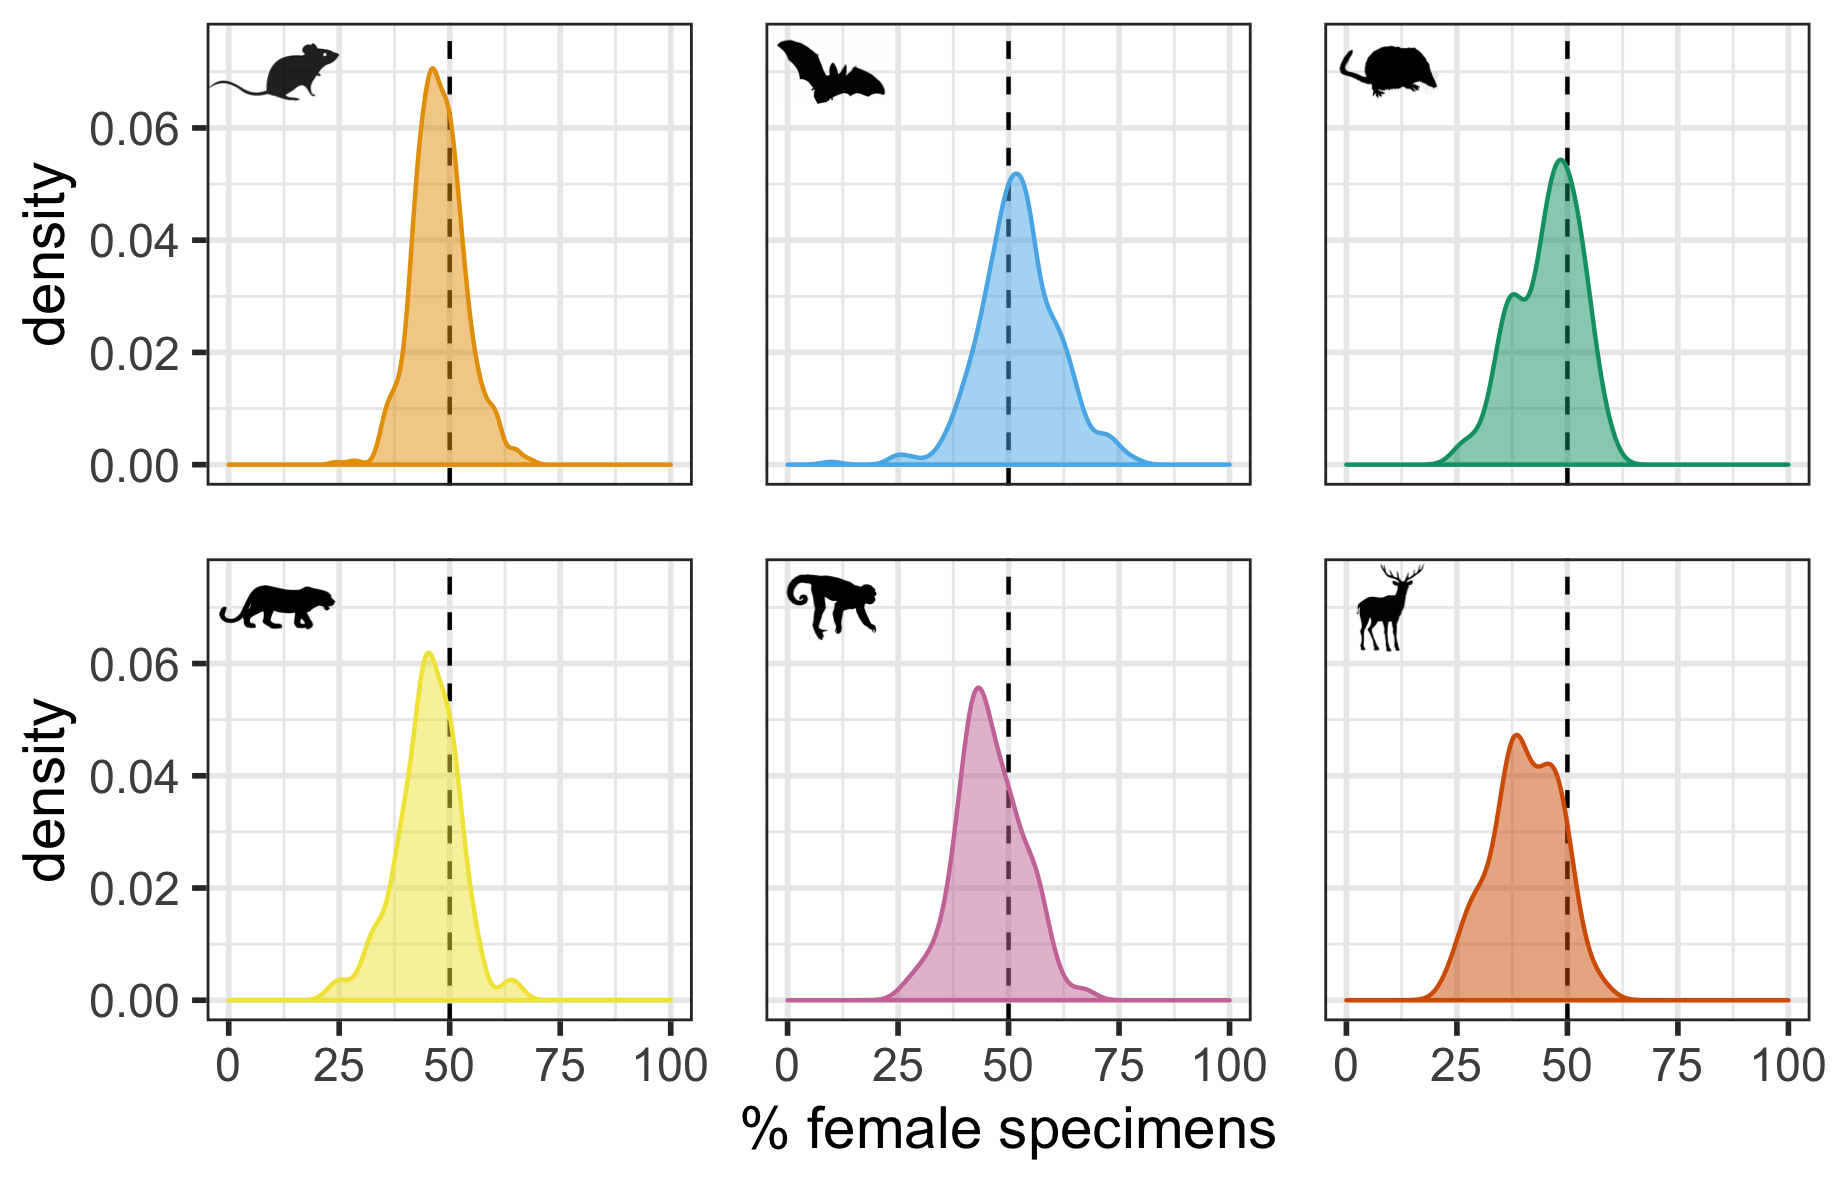
\includegraphics[width = \linewidth]{figures/orders-density-mammals-six.png}
  \caption{Kernel density plots showing the \% female specimens in each species across the six largest orders of mammals (from left to right, top to bottom: Rodentia, Chiroptera, Soricomorpha, Carnivora, Primates, and Artiodactyla). 
  Only species with at least 100 specimens are included. 
  The dashed line represents 50\% female specimens. 
  Silhouettes are from PhyloPic.org contributed by Daniel Jaron (mouse), Yan Wong (bat), Becky Barnes (shrew), Lukasiniho (tiger), Sarah Werning (monkey), and Oscar Sanisidro (deer).
}
  \label{fig-mammal_order_six}
\end{figure}


% figure 3
\newpage
\begin{figure}[h]
 \centering
  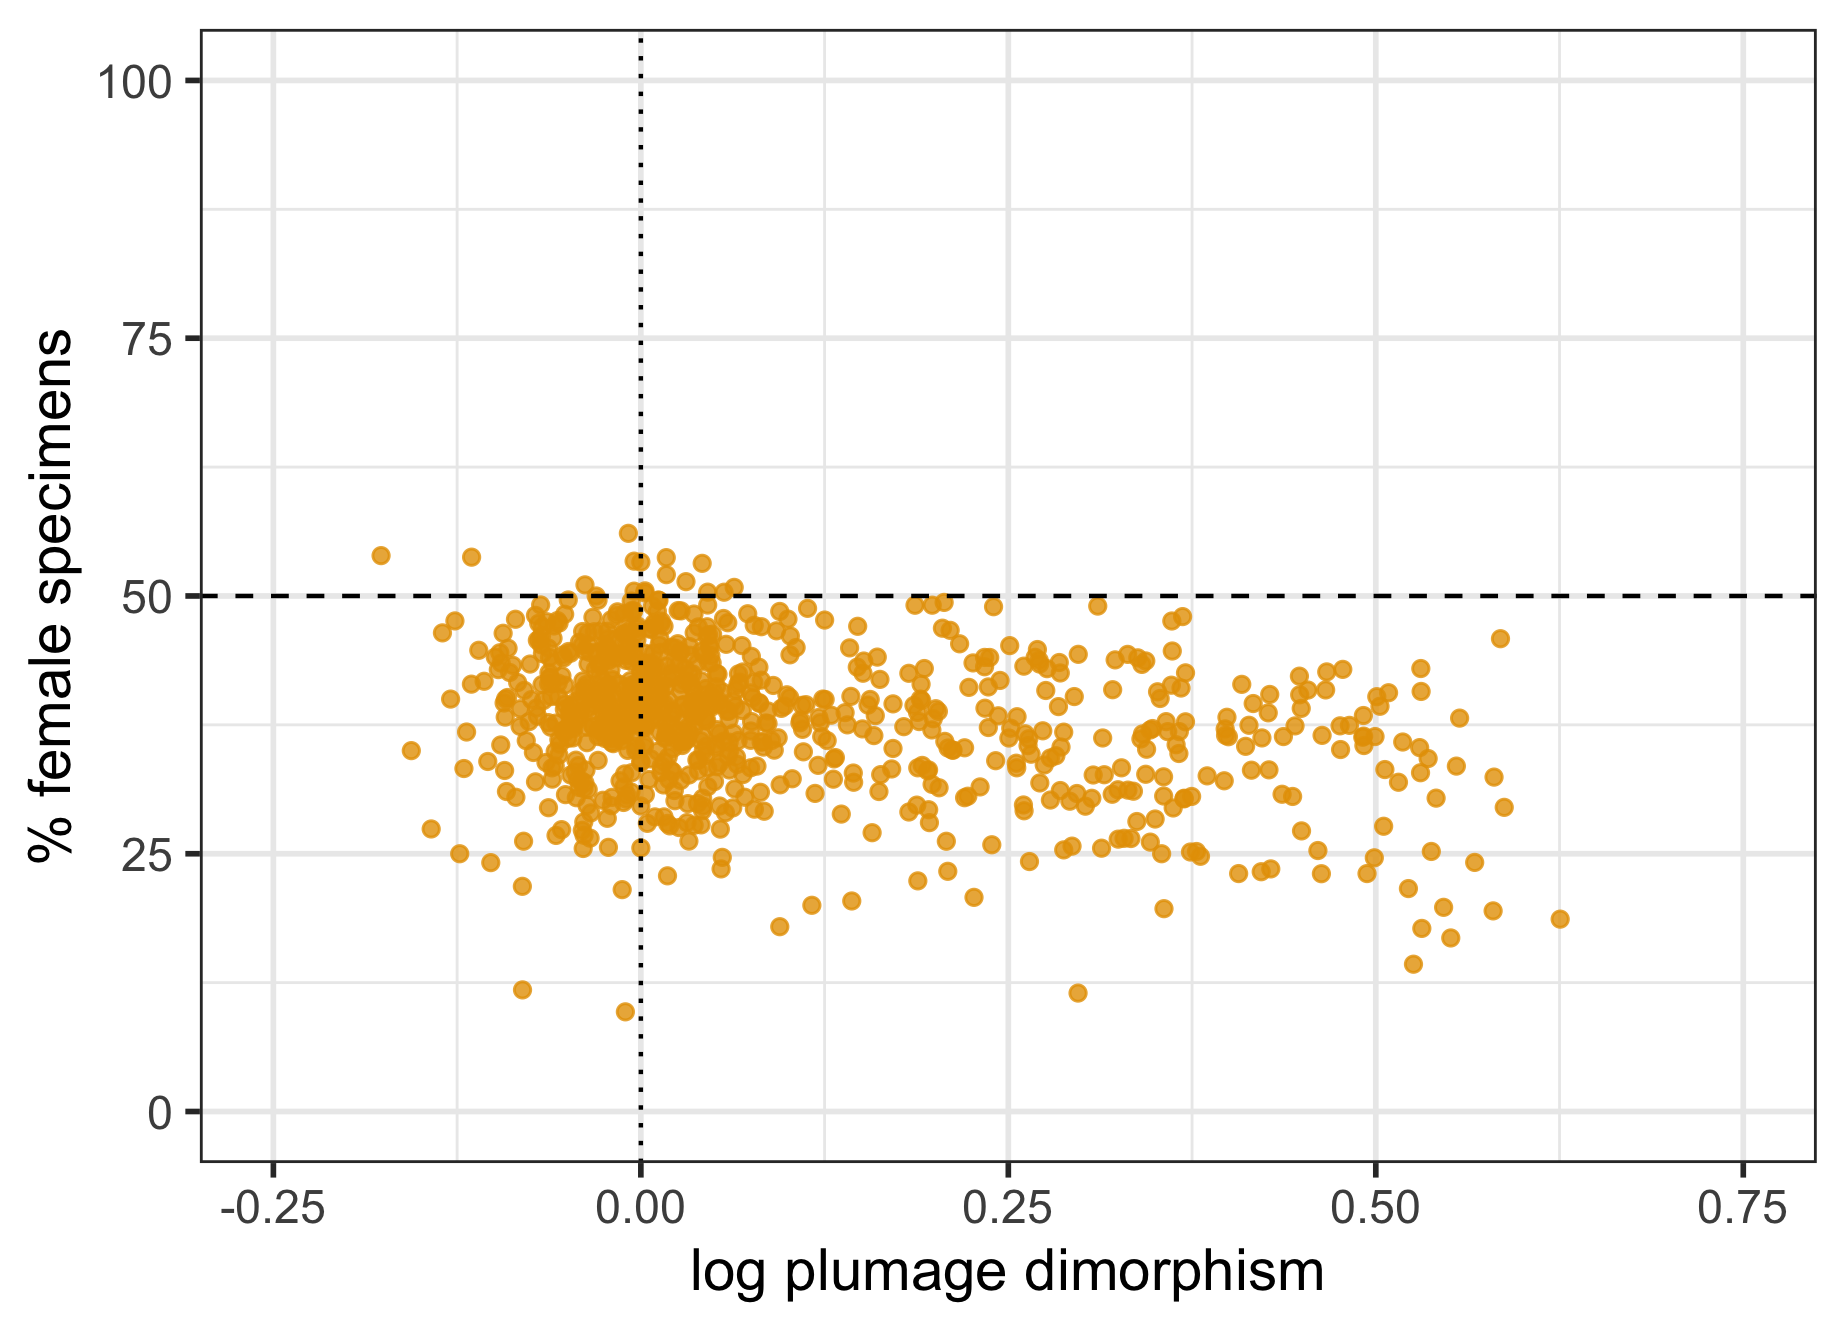
\includegraphics[width = \linewidth]{figures/plumage.png}
  \caption{Relationship between the percentage of female specimens for each species and log plumage dimorphism scores in passerine birds. 
  Only species with at least 100 specimens are included. 
  The dashed line represents 50\% female specimens; the dotted line is the point at which males and females have the same plumage colouration. 
  Plumage dimorphism scores were calculated by dividing male plumage scores by female plumage scores (see Methods). 
}
  \label{fig-plumage}
\end{figure}

% figure 4
\newpage
\begin{figure}[h]
 \centering
  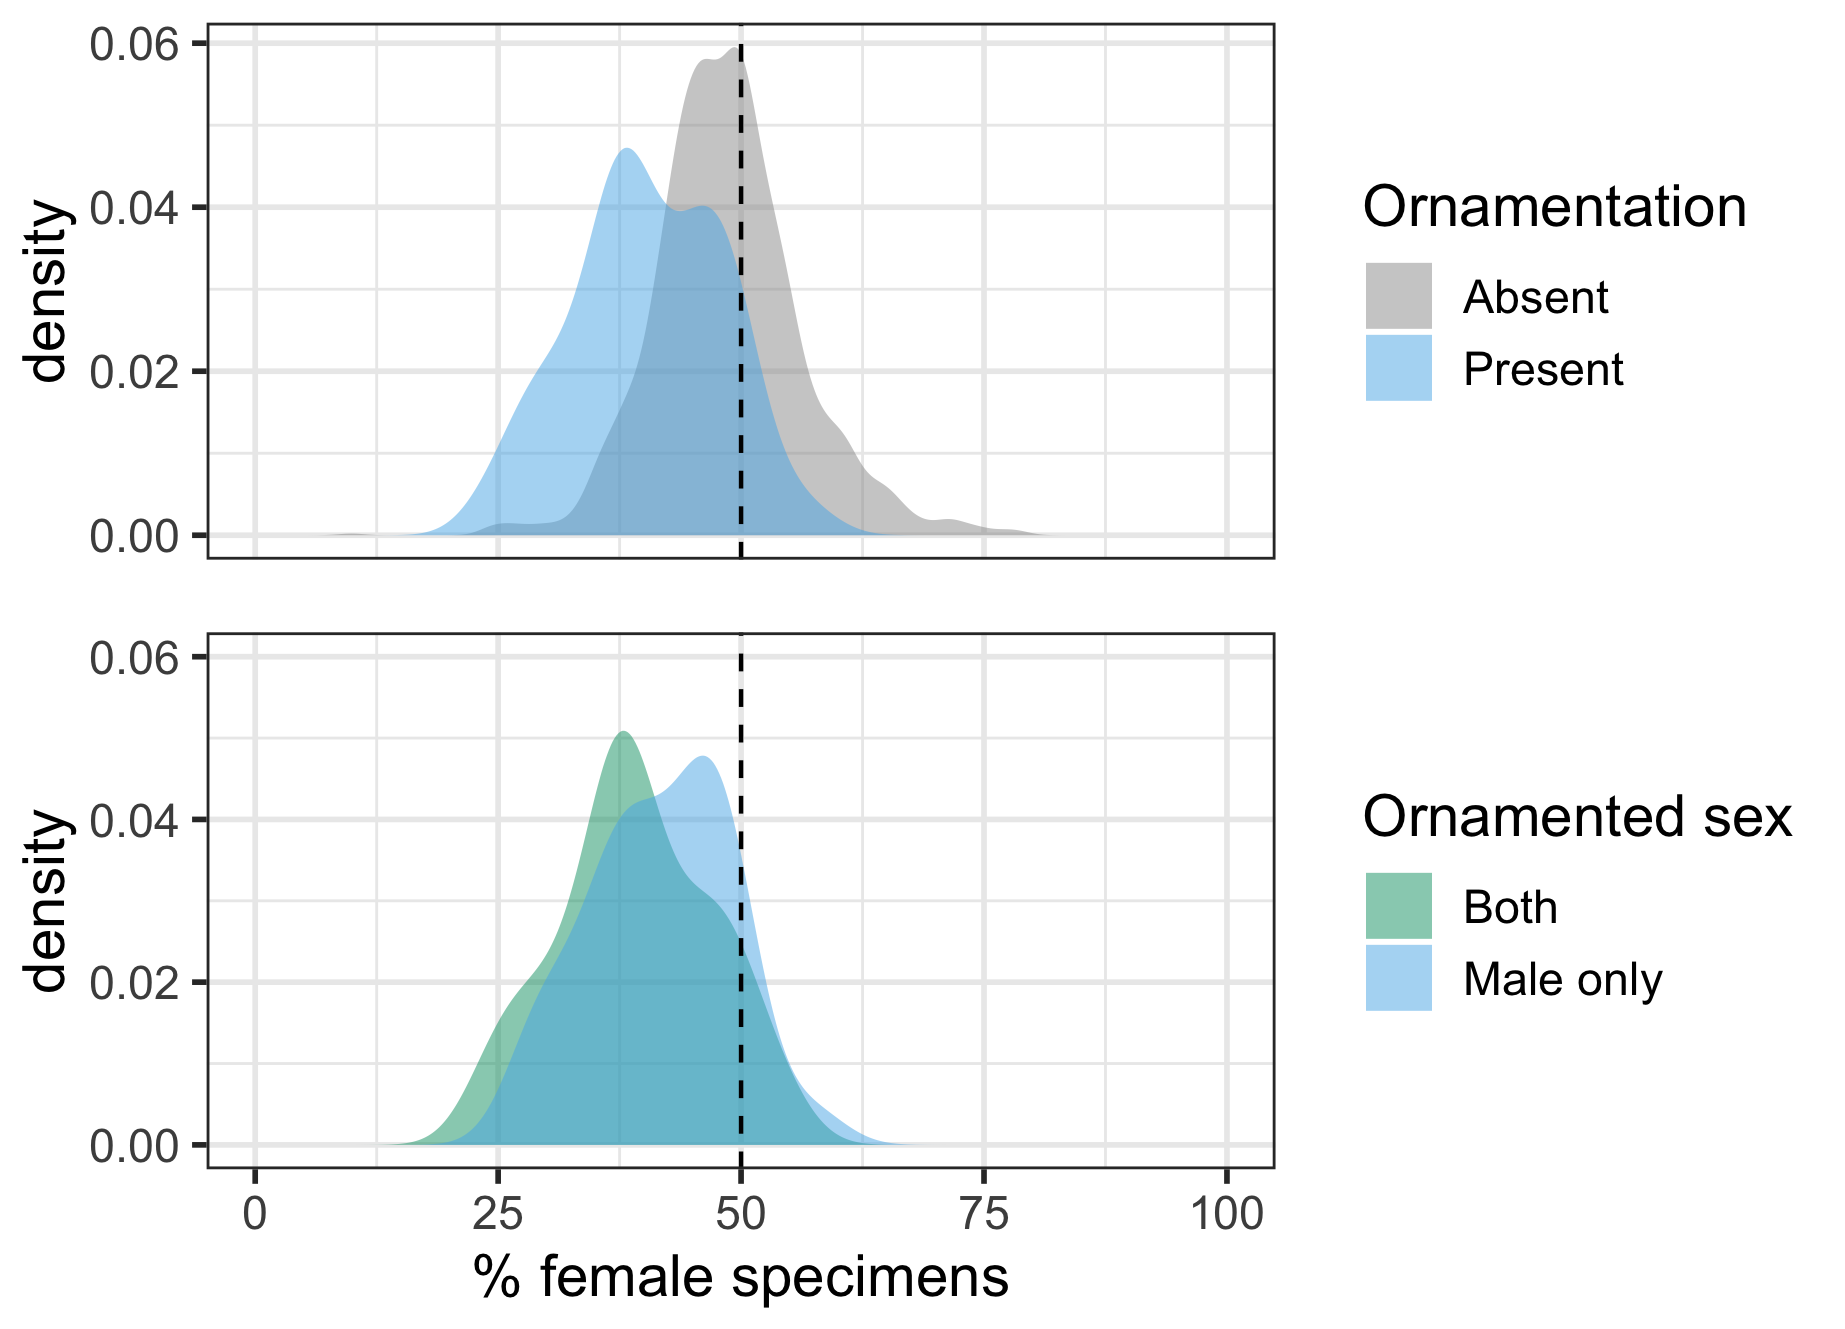
\includegraphics[width = \linewidth]{figures/ornamentation.png}
  \caption{Kernel density plots comparing the \% female specimens in each mammal species where ornaments, i.e. horns, tusks, antlers, manes etc., are present or absent (top panel), and when species have ornaments, whether these are found in both sexes or only males (bottom panel). 
  Only species with at least 100 specimens are included. 
  The dashed line represents 50\% female specimens. 
}
  \label{fig-orn}
\end{figure}

\newpage
\section{Table and figure legends}

Table 1: Prominent uses of natural history specimens and how research outcomes may be influenced by sex biases.

Figure 1: Kernel density plots showing the \% female specimens in each species across the six largest orders of birds (from left to right, top to bottom: Passeriformes, Apodiformes, Piciformes, Psittaciformes, Charadriiformes, and Columbiformes). 
  Only species with at least 100 specimens are included. 
  The dashed line represents 50\% female specimens. 
  Silhouettes are from PhyloPic.org contributed by Ferran Sayol (parrot, hummingbird, tit), Steven Traver (woodpecker) and Alexandre Vong (shorebird).

Figure 2: Kernel density plots showing the \% female specimens in each species across the six largest orders of mammals (from left to right, top to bottom: Rodentia, Chiroptera, Soricomorpha, Carnivora, Primates, and Artiodactyla). 
  Only species with at least 100 specimens are included. 
  The dashed line represents 50\% female specimens. 
  Silhouettes are from PhyloPic.org contributed by Daniel Jaron (mouse), Yan Wong (bat), Becky Barnes (shrew), Lukasiniho (tiger), Sarah Werning (monkey), and Oscar Sanisidro (deer).

Figure 3: Relationship between the percentage of female specimens for each species and log plumage dimorphism scores in passerine birds. 
  Only species with at least 100 specimens are included. 
  The dashed line represents 50\% female specimens; the dotted line is the point at which males and females have the same plumage colouration. 
  Plumage dimorphism scores were calculated by dividing male plumage scores by female plumage scores (see Methods).

Figure 4: Kernel density plots comparing the \% female specimens in each mammal species where ornaments, i.e. horns, tusks, antlers, manes etc., are present or absent (top panel), and when species have ornaments, whether these are found in both sexes or only males (bottom panel). 
  Only species with at least 100 specimens are included. 
  The dashed line represents 50\% female specimens.


\end{document}